\documentclass[english, 11pt]{article}
\usepackage{../notes}
\usepackage{lipsum}

%Global Course Variables
\newcommand{\myCourseCode}{EECS 445}
\newcommand{\myCourseName}{Introduction to Machine Learning}
\newcommand{\myProf}{Honglak Lee}
\newcommand{\myTerm}{Fall 2015}

%Headers
\lhead{\myCourseName}
\rhead{\fancyplain{}{\rightmark}} 

%Footers
\cfoot{\thepage}

\begin{document}
\titleHeader{\myCourseCode}{\myCourseName}{\myProf}{\myTerm}

%Document information
\rule[0.5ex]{1\columnwidth}{.5pt}
Contributors: Max Smith
\begin{center}
	Latest revision: \today
\end{center}
\toc
\abstr{Theory and implementation of state-of-the-art machine learning algorithms for large-scale real-world applications. Topics include supervised learning (regression, classification, kernel methods, neural networks, and regularization) and unsupervised learning (clustering, density estimation, and dimensionality reduction).}

%----------------------------
%Document Begins
%----------------------------
% Unnamed Examples:

\begin{defn}
	A relative path is a path that is referring to your current directory.
\end{defn}

\begin{rem}
	Recall that double quotes do not protect back quotes.
\end{rem}

\begin{exmp}
	$$2+2=3$$
\end{exmp}

With some names:
\begin{defn}[Relative Path]
    A relative path is a path that is referring to your current directory.
\end{defn}

\begin{rem}[Double Quotes]
    Recall that double quotes do not protect back quotes.
\end{rem}

\begin{exmp}[Addition]
    $$2+2=3$$
\end{exmp}

\section{Readings}
	\subsection{Probability Distributions}
	\begin{defn}[Binary Variable]
	Single variable that can take on either 1, or 0; $x\in \{0, 1\}$. We denote $\mu$ ($0\leq\mu\leq 1$) to be the probability that the random binary variable $x=1$
	$$p(x=1|\mu)=\mu$$
	$$p(x=0|\mu)=1-\mu$$
\end{defn}

\begin{defn}[Bernoulli Distribution]
	Probability distribution of the binary variable x, where $\mu$ is the probability $x=1$.
	$$\text{Bern}(x|\mu)=\mu^x(1-\mu)^{1-x}$$
	The distribution has the following properties:
	\begin{itemize}
		\item $\text{E}(x)=\mu$
		\item $\text{Var}(x)=\mu (1-\mu)$
		\item $\mathcal{D}=\{x_1,\ldots ,x_N\} \to p(\mathcal{D} | \mu )=\Pi_{n=1}^{N}p(x_n|\mu)$
		\item Maximum likelihood estimator: $\mu_{ML}=\frac{1}{N}\sum_{n=1}^{N}x_n=\frac{numOfOnes}{sampleSize}$ (aka. sample mean)
	\end{itemize}
\end{defn}

\begin{defn}[Binomial Distribution]
	Distribution of $m$ observations of $x=1$, given a sample size of $N$. 
	$$\text{Bin} (m|N,\mu={\substack{N\\m}}\mu^m (1-\mu )^{N-m}$$\
	\begin{itemize}
		\item $\text{E}(m)=N\mu$
		\item $\text{Var}(m)=N\mu (1-\mu )$
	\end{itemize}
\end{defn}

\subsubsection{The Beta Distribution}
In order to develop a Bayesian treatment for fitting data sets, we will introduce a prior distribution $p(\mu)$.

\begin{itemize}[--]
	\item \textbf{Conjugacy:} when the prior and posterior distributions belong to the same family.
\end{itemize}

\begin{defn}[Beta Distribution]
	$$\text{Beta}(\mu |a,b)=\frac{\Gamma (a+b)}{\Gamma (a)\Gamma (b)}\mu^{a-1} (1-\mu )^{b-1}$$
	Where $\Gamma (x)$ is the gamma function.
	The distribution has the following properties:
	\begin{itemize}
		\item $\text{E}(\mu )=\frac{a}{a+b}$
		\item $\text{Var}(\mu )=\frac{ab}{(a+b)^2 (a+b+1)}$
		\item conjugacy
		\item ${a\to\infty || b\to\infty}\to \text{variance}\\to 0$ 
	\end{itemize}

	Conjugacy can be shown by the distribution by the likelihood function (binomial):
	$$p(\mu |m,l,a,b)\propto \mu^{m+a-1} (1-\mu )^{l+b-1}$$
	Normalized to:
	$$p(\mu |m,l,a,b)= \frac{\Gamma (m+a+l+b)}{\Gamma (m+a)\Gamma (l+b)} \mu^{m+a-1} (1-\mu )^{l+b-1}$$
\end{defn}

\begin{itemize}[--]
	\item \textbf{Hyperparameters:} parameters that control the distribution of the regular parameters.
	\item \textbf{Sequential Approach:} method of learning where you make use of an observation one at a time, or in small batches, and then discard them before the next observatiosn are used. (Can be shown with a Beta, where observing $x=1\to a++, x=0\to b++$, then normalizing)
	\item For a finite data set, the posterior mean for $\mu$ always lies between the prior mean and the maximum likelihood estimate.
	\item A general property of Bayesian learning is when we observe more and more data the uncertainty of the posterior distribution will steadily decrease.
	\item More information and examples of probability distributions can be found in Appendix B of Bishop's `Pattern Recognition and Machine Learning.'
\end{itemize}


	\subsection{Linear Models for Regression}
	\begin{itemize}[--]
	\item \textbf{Linear Regression:} $y(\mathbf{x}, \mathbf{w})=w_0+w_1 x_1+\ldots +w_D x_D$
	\item Limited on linear function of input variables $x_i$
	\item Extend the model with nonlinear functions, where $\phi_j (x)$ are known as basis functions:
		$$y(\mathbf{x}, \mathbf{w})=w_0 +\sum_{j=1}^{M-1}w_j\phi_j (x)$$
	\item $w_0$ allows for any fixed offset in data, and is known as the \textbf{bias parameter}.
	\item Given a dummy variable $\phi_0 (x)=1$, our model becomes:
		$$y(\mathbf{x}, \mathbf{w})=\sum_{j=0}^{M-1}w_j\phi_j (x)=\mathbf{W}^\mathbf{T} \mathbf{\phi} (x)$$
	\item Functions of this form are called \textbf{linear models} because the function is linear in weight.
\end{itemize}

\subsubsection{Maximum likelihood and least squares}
\begin{itemize}[--]
	\item j
\end{itemize}

\section{Stanford Notes}
	\subsection{Linear Regression with One Variable}
	\subsubsection{Model Representation}
\begin{itemize}[--]
	\item Goal is model labelled data (data which we have the correct output for) to a line 
	\item Notation:\begin{description}
		\item[$m$] = number of training examples
		\item[$x$] = input variable/feature
		\item[$y$] = output variable/feature
		\item[$(x,y)$] = one training example
		\item[$(x^{(i)},y^{(i)})$] = $i$th training example (parens indicate index)
	\end{description}

	\item We take a training set, input into a learning algorithm, which returns a hypothesis ($h$) that models the relationship.
	\begin{center}\begin{tikzpicture}[node distance = 2cm, auto]
		%Place nodes
		\node [block] (train) {Training Set};
		\node [block, below of=train] (alg) {Learning Algorithm};
		\node [block, below of=alg] (hyp) {$h$};
		\node [cloud, left of=hyp] (x) {$x$};
		\node [cloud, right of=hyp] (y) {$y$};

		%Draw edges
		\path [line] (train) -- (alg);
		\path [line] (alg) -- (hyp);
		\path [line] (x) -- (hyp);
		\path [line] (hyp) -- (y);
	\end{tikzpicture}\end{center}
	\item $h$ maps from $x$'s to $y$'s ($h(x)=y$).
	\item We need to determine how we want to represent $h$
	\item A simple linear model with one variable for $h$ is: $$h_\theta (x) = \theta_0 + \theta_1 x$$, called \textbf{univariate linear regression}.
\end{itemize}

\subsubsection{Cost Function}
\begin{itemize}[--]
	\item Given a hypothesis: $h_\theta (x) = \theta_0 + \theta_1 x$
	\begin{description}
		\item[$\theta_i's$] = parameters of the model
	\end{description}

	\item We will now discuss how to choose the parameters of our model
	\item Idea: choose $\theta_0, \theta_1$ so that $h_\theta (x)$ is close to $y$ for our training examples $(x,y)$
	\item We want to minimize $\theta_0, \theta_1$ such that $h(x) - y$ is minimal (reminder: $h(x)$ is the guess at the correct value at $y$).
	\item Because we we only are looking to minimize our absolute distance, we square the distance we want to minimize to account for positive and negative differences equally now making our cost function: $(h(x)-y)^2$
	\item However, we don't want to minimize it for just one example, so we do this for every training example: $$\sum_{i=1}^{m}(h_\theta (x^{(i)}) - y^{(i)})^2$$
	\item To make later math easier, we further refine our formula to be half the average: $$\frac{1}{2m}\sum_{i=1}^{m}(h_\theta (x^{(i)}) - y^{(i)})^2$$
	\item This function we created is called our \textbf{cost} function, as it measures how expensively incorrect our current model is, which we will denote with $J$. 
	\item The cost function is dependent on the hypothesis parameters, and our goal is to adjust these parameters to minimize the overrall cost of our model: $$J(\theta_0, \theta_1) = \frac{1}{2m}\sum_{i=1}^{m}(h_\theta (x^{(i)}) - y^{(i)})^2$$
	\item Now our goal is to minimize $J$ over the variables $\theta_0, \theta_1$
\end{itemize}

\subsubsection{Cost Function - Intuition I}
\begin{center}
	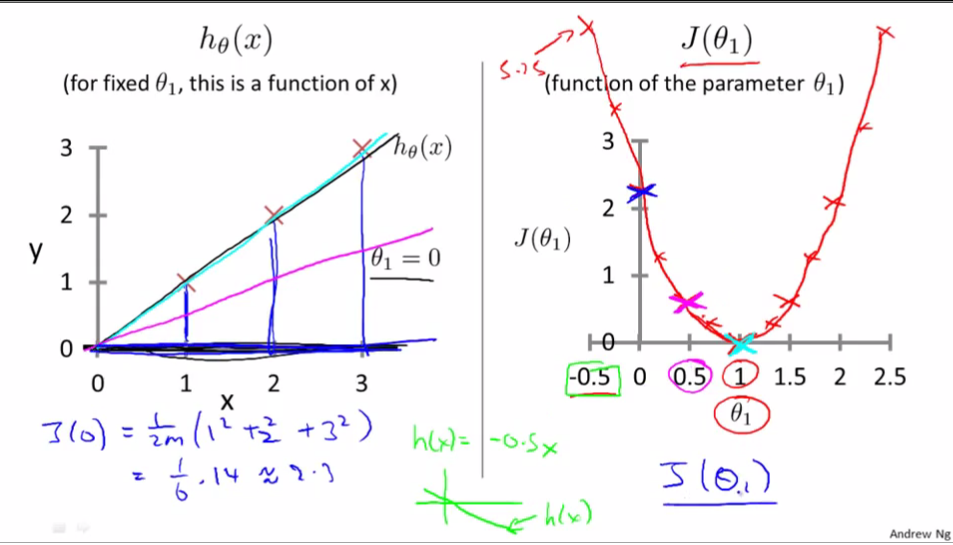
\includegraphics[scale=0.75]{sections/cs229/w1/cost_function.png}
\end{center}
This image shows that for varying parameter values, the cost function changes. In this idealistic example there's a global minimum, the goal of minimized cost, that is very easily followed by a hill-climbing style algorithm.

\subsubsection{Cost Function - Intuition II}
\begin{center}
	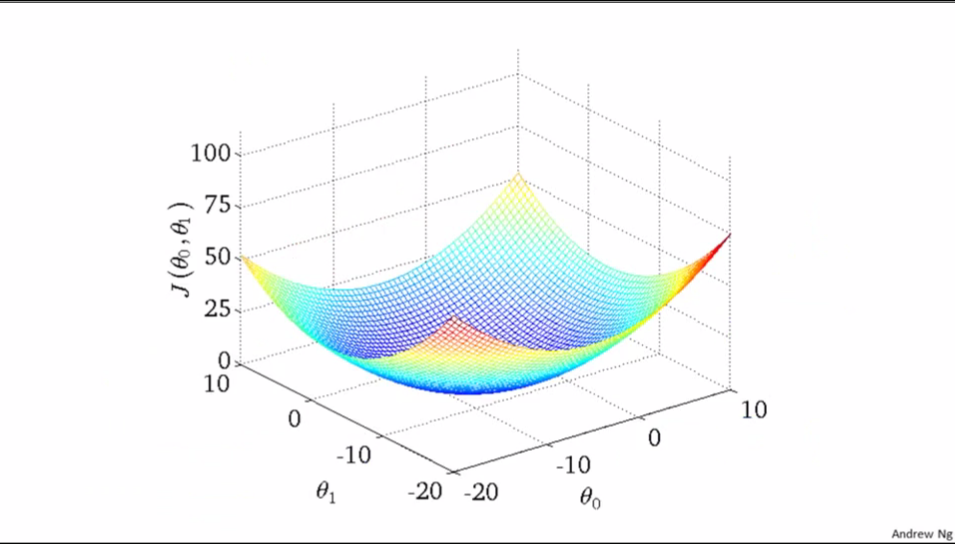
\includegraphics[scale=0.75]{sections/cs229/w1/2d_cost_function.png}
\end{center}
Similarly when you have an additional variable, you want to reach the bottom of this $N$-dimensional hill (note: not all models will have such a perfect hill). 
\begin{itemize}[--]
	\item The gradient gives the direction of maximumal increase on a surface.
	\item We will use a negative gradient to find the `direction' to travel towards the bottom of the hill
	\item Another common way to represent multidimensional cost functions is through contour plots
	\item 
\end{itemize}

	\subsection{Linear Regression with Multiple Variables}
	\subsubsection{Multiple Features}
\begin{itemize}[--]
	\item Instead of just one feature ($x$), we known multiple features ($x_1,\ldots, x_n$). eg. size, number of bedrooms, number of floors, age of home.
	\item $x^{(i)}_j:$ value of feature $j$ in $i^{th}$ training example
	\item Now our hypothesis must account for multiple features: 
		$$h_\theta (x)=\theta_0 + \theta_1 x_1 + \ldots \theta_n x_n$$
	\item Again we define $x_0 = 1$ to simplify future math ($x^{(i)}_0=1$).
	$$x=\begin{bmatrix} x_1\\ \vdots\\ x_n\end{bmatrix}\in \mathbb{R}^{n+1}\text{,  }
		\theta = \begin{bmatrix}\theta_0 \\ \vdots\\ \theta_n\end{bmatrix}\in\mathbb{R}^{n+1}$$
	\item Transposing the $\theta$ vector given our assumption for $x_0^{(i)}$ allows us to simplify our hypothesis into:
		$$h_\theta (x) = \theta^{T}x$$
\end{itemize}

\subsubsection{Gradient Descent for Multiple Variables}
\begin{itemize}[--]
	\item Repeat until convergence ($j=0,\ldots, n$): 
		$$\theta_j := \theta_j \alpha\frac{1}{m}\sum_{i=1}^{m}(h(x^{(i)}-y^{(i)}))x^{(i)}_j$$
	\item This is a valid generalization of the previous formula because of our base case $x^{(i)}_0=1$
\end{itemize}

\subsubsection{Gradient Descent in Practice I - Featuer Scaling}
\begin{itemize}[--]
	\item \textbf{Feature scaling:} if features are on similar scales then we converge more quickly
	\item Your parameters will oscillate along the larger ranged parameter making it's way much slower towards the center (in the case of two variables); whereas, if both axis were equal then you don't have a worst case to fret about
	\begin{center}
		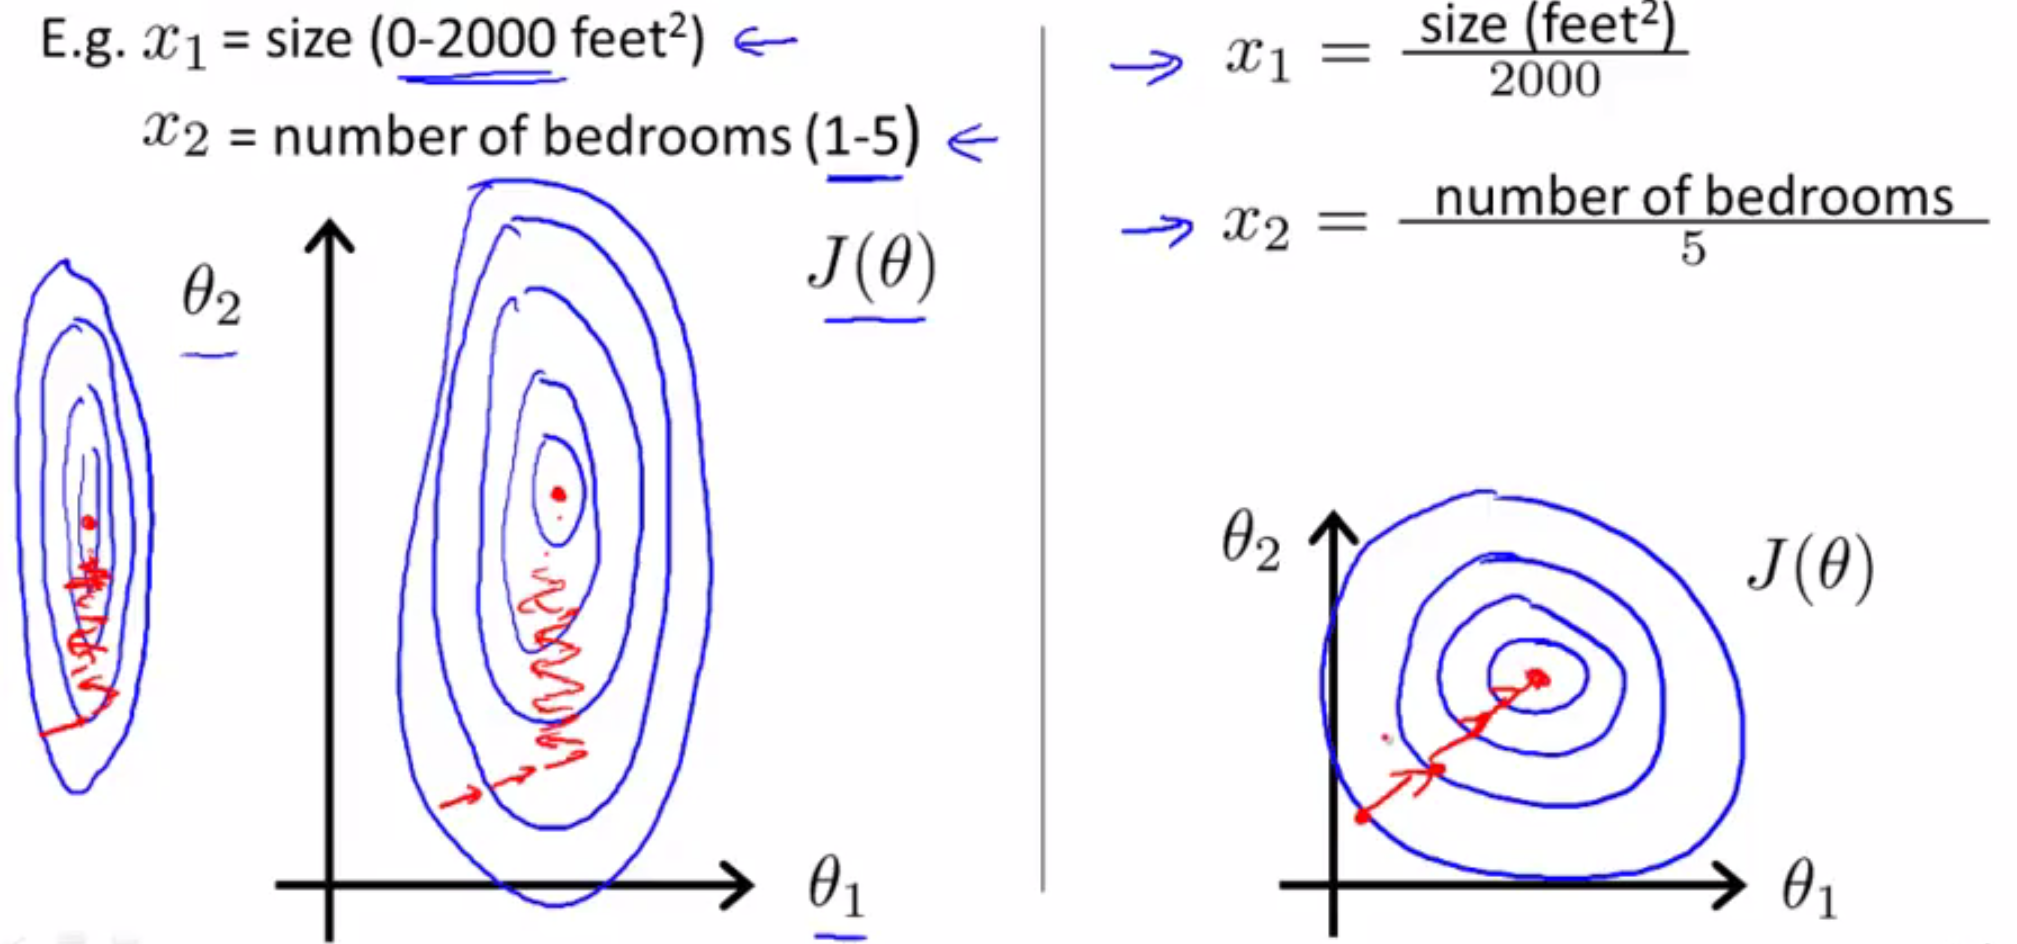
\includegraphics[scale=0.25]{sections/cs229/w2/feature_scaling.png}
	\end{center}

	\item Typically, we want to scale each feature into approximately a $-1\leq x_i \leq 1$ range (same order of magnitude).
	\item \textbf{Mean normalization:} replacing $x_i$ with $x_i-\mu_i$ to make features have approximately zero mean (does not apply to $x_0=1$).
	\item Combining mean normalization and feature scaling we assign $x_i := \frac{x_i-\mu_i}{range_i}$

\end{itemize}

\subsubsection{Gradient Descent in Practice II - Learning Rate}
\begin{itemize}[--]
	\item To ensure gradient descent is working correctly, plot the cost function against the number of iterations. It should converge towards 0, decreasing at every iteration.
	\item The number of iterations required can vary widely for different applications
	\item You can create an automatic convergence test to ensure appropriately ending of gradient descent by checking if the difference between two iterations $\epsilon$ is below a threshold.
	\item If there is any increase in slope, use a smaller $\alpha$
	\item For sufficiently small $\alpha$, $J(\theta )$ should decrease on every iteration
	\item But if $\alpha$ is too small, gradient descent an be slow to converge
	\item To choose $\alpha$ try: $\ldots, 0.001, 0.003, 0.01, 0.03, 0.1, 0.3, 1,\ldots$
\end{itemize}

\subsubsection{Features and Polynomial Regression}
\begin{itemize}[--]
	\item Suppose we have a housing price prediction: $h(x)=\theta_0 + \theta_1 (frontage)+\theta_2 (depth)$
	\item We can define a new feature $(area)=(frontage)(depth)$, that we can use in a new hypothesis $h(x)=\theta_0+\theta_1 (area)$
	\item We can map these hypothesis of more complex features into a linear regression problem: 
	\begin{align*}
		h(x)&=\theta_0 + \theta_1 x_1 + \theta_2 x_2 + \theta_3 x_3    
  		  	&=\theta_0 + \theta_1 (size) + \theta_2 (size)^2 + \theta_3 (size)^3
	\end{align*}

	\item If your features are like those chosen, then feature scaling is very important
	\item There are many more choices for modifications to our features (such as: $\sqrt{}$).
	\item Trying new features can allow you to have a more appropriate model
\end{itemize}

\subsubsection{Normal Equations}
\begin{itemize}[--]
	\item The \textbf{normal equation} allows us to solve for $\theta$ analytically (without iterations)
	\item Intuition: $J(\theta) = a\theta^2+b\theta+c$
	In previous calculus classes you would find the minimum by taking the derivative set equal to 0 and solving for $\theta$. 
	\item This can be extended with partial fractions and solving for every $\theta_j\in\theta$. $$\frac{\partial}{\partial\theta_j}J(\theta)=\ldots=0 \text{    (for every}j\text{)}$$
	\item We construct a matrix from the features and a vector from the solutions as so ($n$ features, $m$ examples):

	\[X=\begin{bmatrix}
		x_0^{(1)} & x_1^{(1)} & \dots & x_n^{(1)} \\
		x_0^{(2)} & x_1^{(2)} & \dots & x_n^{(2)} \\
		\vdots & \vdots & \ddots & \vdots \\
		x_0^{(m)} & x_1^{(m)} & \dots x_n^{(m)} 
	\end{bmatrix} \in \mathbb{R}^{m\times (n+1)}
	 \]

	 \[
	y=\begin{bmatrix}
		y^{(1)} \\
		y^{(2)} \\
		\vdots \\
		y^{(m)}
	\end{bmatrix}\in \mathbb{R}^{m\times 1}
	 \]

	 \item We can then represent the $\theta$ by the \textbf{normal equation} $$\theta = (X^{T}X)^{-1}X^{T}y$$\
	 \item $X$ is entitled the \textbf{design matrix}
	 \item Normal equation does not perform well with a large $n$ due to the computation $(X^{T}X)^{-1}\in\mathbb{n\times n}$ which is typically $\O{n^3}$
\end{itemize}

	\subsection{Logistic Regression}
	\subsubsection{Multiple Features}
\begin{itemize}[--]
	\item 
\end{itemize}



	\subsection{Regularization}
	\subsubsection{The Problem of Overfitting}
\begin{itemize}[--]
	\item \textbf{Underfitting}: when a model cannot capture the underlying trend of the data ("high bias")
	\item \textbf{Overfitting}: when a model captures the noise of the data ("high variance")
	\item \textbf{Generalize}: fails to fit to new examples
	\item Overfitting's poor generalization results in low costs not always being correct
	\begin{center}
		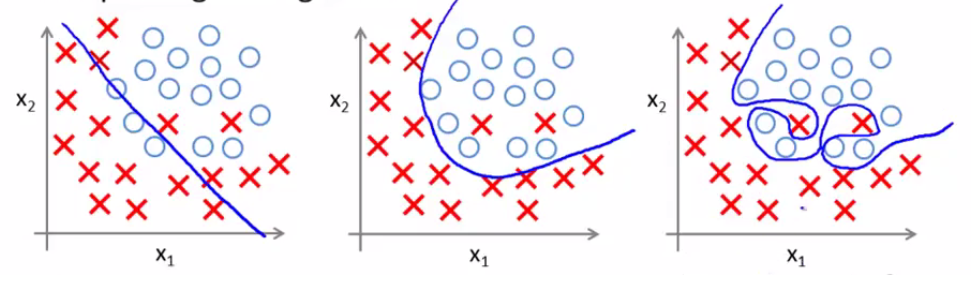
\includegraphics[scale=0.5]{sections/cs229/w4/over-under.png}
	\end{center}

	\item If we have too many features for very little data, overfitting can easily become a big problem.
	\item Options:
	\begin{itemize}
		\item Reduce number of features
		\begin{itemize}
			\item Manually select which features to keep
			\item Model selection algorithm (later in course)
		\end{itemize}
		\item Regularization
		\begin{itemize}
			\item Keep all the features, but reduce magnitude/values of parameters $\theta_j$
			\item Works well when we have a lot of features, each of which contributes a bit to predicting $y$
		\end{itemize}
	\end{itemize}

\end{itemize}

\subsubsection{Cost Function}
\begin{itemize}[--]
	\item Having smaller values for parameters $\theta_0, \theta_1, \ldots, \theta_n$
	\begin{itemize}[--]
		\item ``Simpler'' hypothesis
		\item Less prone to overfitting
	\end{itemize}

	\item To exemplify lets consider the housing scenario:
	\begin{itemize}[--]
		\item Features: $x_1,\ldots, x_100$
		\item Paremeters: $\theta_0, \ldots, \theta_100$
		\item We don't know which ones are complex to shrink, so we modify the cost function to shrink every parameter
		$$J(\theta )=\frac{1}{2m}(\sum_{i=1}^{m}(h(x^{(i)}-y^{(i)})^2 + \lambda\sum_{i=1}^{n}\theta_j^2)$$
		\item We don't penalize $\theta_0$ by convention, because it's a constant and makes very little difference
	\end{itemize}

	\item $\lambda$ is called the regularization parameter. It controls the trade off of fitting the training set well and keeping the parameters small and simple to prevent overfitting
	\item If $\lambda$ is set to be very large we will penalize all the paramters extremely highly resulting which will result in all by the constant being close to zero (fits to a horizontal line). ``Underfit''
\end{itemize}

\subsubsection{Regularized Linear Regression}
\begin{itemize}[--]
	\item Using the new regularized linear regression cost function from the previous section we can now update our gradient descent algorithm to encorporate this modification:
		$$\theta_0 := \theta_0 - \alpha\frac{1}{m}\sum_{i=1}^{m} (h(x^{(i)})-y^{(i)})x_0^{(i)}$$
		$$\theta_j := \theta_j - \alpha ( \frac{1}{m}\sum_{i=1}^{m}(h(x^{(i)})-y{(i)})x)j^{(i)} +\frac{\lambda}{m}\theta_j )$$

	\item The $\theta_j$ $(j=1,\ldots, n)$ term can also be written:
		$$\theta_j := \theta_j (1-\alpha\frac{\lambda}{m}) - \alpha\frac{1}{m}\sum_{i=1}^{m}(h(x^{(i)}) - y^{(i)})x_j^{(i)}$$

	\item The term $(1-\alpha\frac{\lambda}{m})$ is typically $<1$, so this results in shrinking $\theta_j$ by multiplying by a value $<1$, and then performing the same gradient descent function
	\item We also had the normal equation to solve the same problem, and it can also be updated for regularization:
		$$\theta = (X^{T}X+\lambda \left[ \begin{smallmatrix}
			0 & & &\\
			& 1 & &  \\
			& & \ldots & \\
			& & & 1 
		\end{smallmatrix}\right] )X^{T}y$$

	\item Suppose $m\leq n$ then $(X^{T}X)$ will be non-invertible/singular
	\item Regularization will take care of this flaw so long as $\lambda > 0$
\end{itemize}

\subsubsection{Regularized Logistic Regression}
\begin{itemize}[--]
	\item We can also regularize logistic regression in a similar manner
		$$\theta_0 := \theta_0 - \alpha\frac{1}{m}\sum_{i=1}^{m} (h(x^{(i)})-y^{(i)})x_0^{(i)}$$
		$$\theta_j := \theta_j - \alpha ( \frac{1}{m}\sum_{i=1}^{m}(h(x^{(i)})-y{(i)})x)j^{(i)} +\frac{\lambda}{m}\theta_j )$$
		$$h(x)=\frac{1}{1+e^{-\theta^{T}x}}$$
\end{itemize}

% \section{Introduction and Overview}
% \section{Supervised Learning: Regression}
% \section{Supervised Learning: Classification}
% \section{Kernel Methods}
% \section{Regularization and Model Selection}
% \section{Advice on using ML Algorithms}
% \section{Neural Networks}
% \section{Unsupervised Learning}
% \section{Gaussian Process}
% \section{Ensemble Methods}
% \section{Sequence Modeling}
% \section{Learning Theory}

\end{document}